\documentclass{article}\usepackage[]{graphicx}\usepackage[]{color}
% maxwidth is the original width if it is less than linewidth
% otherwise use linewidth (to make sure the graphics do not exceed the margin)
\makeatletter
\def\maxwidth{ %
  \ifdim\Gin@nat@width>\linewidth
    \linewidth
  \else
    \Gin@nat@width
  \fi
}
\makeatother

\definecolor{fgcolor}{rgb}{0.345, 0.345, 0.345}
\newcommand{\hlnum}[1]{\textcolor[rgb]{0.686,0.059,0.569}{#1}}%
\newcommand{\hlstr}[1]{\textcolor[rgb]{0.192,0.494,0.8}{#1}}%
\newcommand{\hlcom}[1]{\textcolor[rgb]{0.678,0.584,0.686}{\textit{#1}}}%
\newcommand{\hlopt}[1]{\textcolor[rgb]{0,0,0}{#1}}%
\newcommand{\hlstd}[1]{\textcolor[rgb]{0.345,0.345,0.345}{#1}}%
\newcommand{\hlkwa}[1]{\textcolor[rgb]{0.161,0.373,0.58}{\textbf{#1}}}%
\newcommand{\hlkwb}[1]{\textcolor[rgb]{0.69,0.353,0.396}{#1}}%
\newcommand{\hlkwc}[1]{\textcolor[rgb]{0.333,0.667,0.333}{#1}}%
\newcommand{\hlkwd}[1]{\textcolor[rgb]{0.737,0.353,0.396}{\textbf{#1}}}%
\let\hlipl\hlkwb

\usepackage{framed}
\makeatletter
\newenvironment{kframe}{%
 \def\at@end@of@kframe{}%
 \ifinner\ifhmode%
  \def\at@end@of@kframe{\end{minipage}}%
  \begin{minipage}{\columnwidth}%
 \fi\fi%
 \def\FrameCommand##1{\hskip\@totalleftmargin \hskip-\fboxsep
 \colorbox{shadecolor}{##1}\hskip-\fboxsep
     % There is no \\@totalrightmargin, so:
     \hskip-\linewidth \hskip-\@totalleftmargin \hskip\columnwidth}%
 \MakeFramed {\advance\hsize-\width
   \@totalleftmargin\z@ \linewidth\hsize
   \@setminipage}}%
 {\par\unskip\endMakeFramed%
 \at@end@of@kframe}
\makeatother

\definecolor{shadecolor}{rgb}{.97, .97, .97}
\definecolor{messagecolor}{rgb}{0, 0, 0}
\definecolor{warningcolor}{rgb}{1, 0, 1}
\definecolor{errorcolor}{rgb}{1, 0, 0}
\newenvironment{knitrout}{}{} % an empty environment to be redefined in TeX

\usepackage{alltt}

\usepackage[english]{babel}
\usepackage{graphicx}
\usepackage{fancyref}
\usepackage{hyperref}
\usepackage[scale=2]{ccicons}
\usepackage{url}
\usepackage{fancyhdr}



\title{Exercises non-parametric methods for within designs}
\author{St\'ephanie M. van den Berg}
\IfFileExists{upquote.sty}{\usepackage{upquote}}{}
\begin{document}

\maketitle






\section{Exercises}


A researcher is interested in the relationship between mood and day of the week: are people generally moodier on Monday than on Wednesday or Friday?

Below we see the data on four people that rated their mood from 1 (very moody) to 10 (not moody at all) on three separate days in a week in February: Day 1 is Monday, day 2 is Wednesday and day 3 is Friday:

\begin{knitrout}
\definecolor{shadecolor}{rgb}{0.969, 0.969, 0.969}\color{fgcolor}
\begin{tabular}{r|r|r}
\hline
ID & Day & Mood\\
\hline
1 & 1 & 3\\
\hline
1 & 2 & 5\\
\hline
1 & 3 & 8\\
\hline
2 & 1 & 4\\
\hline
2 & 2 & 7\\
\hline
2 & 3 & 6\\
\hline
3 & 1 & 2\\
\hline
3 & 2 & 4\\
\hline
3 & 3 & 1\\
\hline
4 & 1 & 9\\
\hline
4 & 2 & 5\\
\hline
4 & 3 & 3\\
\hline
\end{tabular}


\end{knitrout}

\begin{enumerate}

\item Put the data into wide format, and think of appropriate variable names
\\
 \\
 \begin{tabular}{llrrrr}
   & \dots & \dots  & \dots & \dots  & \dots  \\ \hline
  & \dots & \dots  & \dots & \dots  & \dots  \\
  & \dots & \dots  & \dots & \dots  & \dots  \\
  & \dots & \dots  & \dots & \dots  & \dots  \\
  & \dots & \dots  & \dots & \dots  & \dots  \\
  & \dots & \dots  & \dots & \dots  & \dots  \\
  & \dots & \dots  & \dots & \dots  & \dots  \\
  & \dots & \dots  & \dots & \dots  & \dots  \\
  & \dots & \dots  & \dots & \dots  & \dots  \\
  & \dots & \dots  & \dots & \dots  & \dots  \\
  & \dots & \dots  & \dots & \dots  & \dots  \\
  & \dots & \dots  & \dots & \dots  & \dots  \\
  & \dots & \dots  & \dots & \dots  & \dots  \\
 \end{tabular}
\\
\\
\item Rank these data row-wise: for each row determine the lowest mood (1), the second lowest mood (2) and the highest mood score (3)
\\
 \\
 \begin{tabular}{llrrrr}
   & \dots & \dots  & \dots & \dots  & \dots  \\ \hline
  & \dots & \dots  & \dots & \dots  & \dots  \\
  & \dots & \dots  & \dots & \dots  & \dots  \\
  & \dots & \dots  & \dots & \dots  & \dots  \\
  & \dots & \dots  & \dots & \dots  & \dots  \\
  & \dots & \dots  & \dots & \dots  & \dots  \\
  & \dots & \dots  & \dots & \dots  & \dots  \\
  & \dots & \dots  & \dots & \dots  & \dots  \\
  & \dots & \dots  & \dots & \dots  & \dots  \\
  & \dots & \dots  & \dots & \dots  & \dots  \\
  & \dots & \dots  & \dots & \dots  & \dots  \\
  & \dots & \dots  & \dots & \dots  & \dots  \\
  & \dots & \dots  & \dots & \dots  & \dots  \\
 \end{tabular}
\\
\\
\item Determine the column sums: the sum of the ranks for Monday, Wednesday and Friday.
\item How many rows do you have ($N$) and how many columns of data do you have ($k$)?
\item Compute $F_r$.
\item Copy the data into SPSS and run Friedman's test. Should you ask for an exact $p$-value? Provide the syntax.
\item Suppose you get the SPSS output in Figure \ref{fig:friedmanmood1}. What would your conclusion be regarding the research question about the relationship between moodiness and the day of the week?

\begin{figure}[h]
    \begin{center}
       \includegraphics[scale=0.8, trim={0cm 21cm 0cm 0cm}]{/Users/stephanievandenberg/Dropbox/Statistiek_Onderwijs/Data" "Analysis/spss" "examples" "nonparmixed/friedmanmood1.pdf}
    \end{center}
    \caption{SPSS output of a Friedman test.}
    \label{fig:friedmanmood1}
\end{figure}

\item
In this data set, for which day did we observe the personal best mood? How many of the individuals showed their best mood on that day?


\item
A linear mixed model was run on this data set. When checking model assumptions, we saw the graphs in Figures \ref{fig:nonparmixed_11a} and \ref{fig:nonparmixed_11b}. Based on these, would you prefer to stick to the Friedman's test for this data set, or would you prefer to report a linear mixed model? Explain your answer.


\begin{knitrout}
\definecolor{shadecolor}{rgb}{0.969, 0.969, 0.969}\color{fgcolor}\begin{figure}

{\centering 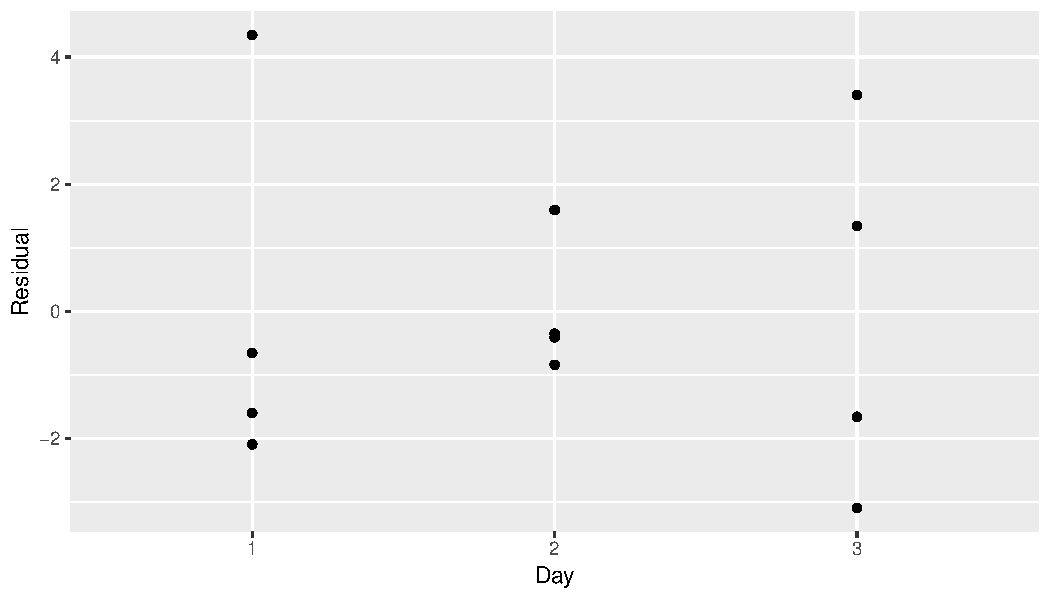
\includegraphics[width=\maxwidth]{figure/nonparmixed_11a-1} 

}

\caption[Residual plot after a linear mixed model analysis]{Residual plot after a linear mixed model analysis.}\label{fig:nonparmixed_11a}
\end{figure}


\end{knitrout}

\begin{knitrout}
\definecolor{shadecolor}{rgb}{0.969, 0.969, 0.969}\color{fgcolor}\begin{figure}

{\centering 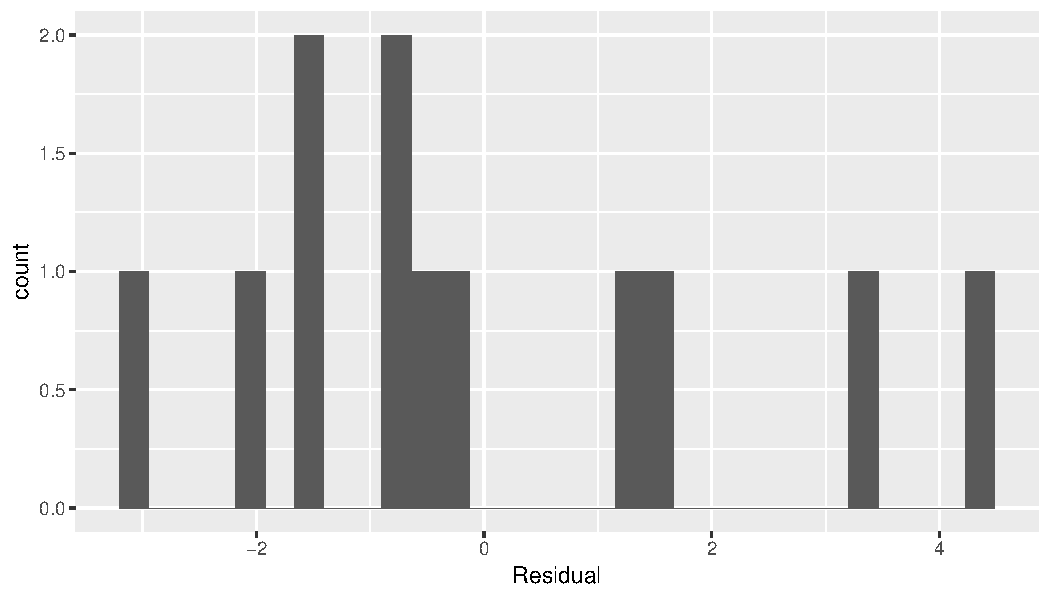
\includegraphics[width=\maxwidth]{figure/nonparmixed_11b-1} 

}

\caption[Residual plot after a linear mixed model analysis]{Residual plot after a linear mixed model analysis.}\label{fig:nonparmixed_11b}
\end{figure}


\end{knitrout}


\item Could you have performed a Wilcoxon test on these data? Why so, or why not?

\end{enumerate}


\subsection{Answers}


\begin{enumerate}

\item
The raw data in wide format:
\begin{knitrout}
\definecolor{shadecolor}{rgb}{0.969, 0.969, 0.969}\color{fgcolor}
\begin{tabular}{r|r|r|r}
\hline
ID & Mood\_1 & Mood\_2 & Mood\_3\\
\hline
1 & 3 & 5 & 8\\
\hline
2 & 4 & 7 & 6\\
\hline
3 & 2 & 4 & 1\\
\hline
4 & 9 & 5 & 3\\
\hline
\end{tabular}


\end{knitrout}

\item
The row-wise ranked data:
\begin{knitrout}
\definecolor{shadecolor}{rgb}{0.969, 0.969, 0.969}\color{fgcolor}
\begin{tabular}{r|r|r|r}
\hline
ID & Mood\_1 & Mood\_2 & Mood\_3\\
\hline
1 & 1 & 2 & 3\\
\hline
2 & 1 & 3 & 2\\
\hline
3 & 2 & 3 & 1\\
\hline
4 & 3 & 2 & 1\\
\hline
\end{tabular}


\end{knitrout}
\item Day 1: 7, Day 2: 10 and Day3: 7.
\item $N=4$ and $k=3$
\item

\begin{eqnarray}
F_r &=& \left[  \frac{12}{4 \times  3(3+1)} \times (7^2 + 10^2 + 7^2)      \right] - 3 \times 4 (3+1) \nonumber \\
  &=&   \left[  \frac{12}{48} \times  198      \right] - 48 = 1.50  \nonumber
\end{eqnarray}

\item

\begin{verbatim}
NPAR TESTS
/FRIEDMAN=  Mood_1   Mood_2    Mood_3
/METHOD=Exact.
\end{verbatim}

\item
\begin{quotation}
We found no significant effect of day of the week on mood, $F_r=1.50, p=0.65$, so the null-hypothesis of equal mood during the week is not rejected. Note however that the sample size was extremely small (12 data points), so even if there is a real relationship between mood and day of the week, there was little chance to find evidence of that in this data set.
\end{quotation}

\item The highest column sum of the ranks was found for day 2, which was Wednesday. So in this data set we saw that the four individuals generally showed their personal highest mood score on Wednesday. Actually, 2 persons out of 4 showed their highest score (rank 3) on Wednesday (ID=2 and ID=3).

\item The plots suggests that the variance of the residuals is very small for the second day, compared to the other two days. The distribution is also hardly normal. But it is hard to tell whether the assumptions are reasonable, since there are so few data points. It would therefore be safest to report a Friedman test.

\item A Wilcoxon test can only be performed on two measures, say Monday and Wednesday data, or Monday and Friday data. You could not test the null-hypothesis of the same moods on three days with a Wilcoxon test.

\end{enumerate}



\end{document}


